%%
%% $Id$
%%
%% Copyright (c) 2007-2008 Christian Fehler
%% Copyright (c) 2007-2008 Benjamin Mies
%%


\chapter{Interaktion}\label{Interaction}

In diesem Kapitel werden die Interaktionen mit dem Benutzer erläutert. Ein
wichtiger Aspekt der Interaktionen ist, dass der Benutzer angezeigt bekommt,
wenn er etwas falsches eingeben hat. Ein weiterer Punkt ist, dass der Benutzer
bei einem nicht deterministischen Kellerautomaten auswählen muss, welchen
Übergang der Automat machen soll, da dieser das im Allgemeinen nicht erkennen
kann.


\section{Fehler und Warnung}

Es war uns bei der Umsetzung des \gtitools sehr wichtig, dass der Benutzer sehr
viele Fehler machen kann, ohne dass er durch eine Validierung eingeschränkt wird.
Eine Ausnahme von diesem Konzept bilden die in Kapitel \ref{Parser} beschriebenen
Parser, da eine falsche Eingabe dort nicht anständig durch das Anzeigen von
Fehlern bzw. Warnungen behandelt hätte werden können.\vspace{10pt}

Der Hauptgrund für die Auswahl dieser Strategie war, dass der Benutzer durch das
fehlerhafte Eingeben bzw. durch das Beheben der Fehler hoffentlich mehr lernt,
als wenn er die Eingaben gar nicht erst hätte machen können. In diesem Abschnitt
werden die verschiedenen Fehler und Warnungen beschrieben, die bei Grammatiken und
Automaten auftreten können.


\subsection{Grammatik}

Im folgenden möchten wir auf die Fehler und Warnungen eingehen, welche bei dem
Validierungsvorgang einer Grammatik auftreten können.\vspace{10pt}

Als Validierungsfehler zählt, unter anderem, wenn die gleiche Produktion mehrfach
angelegt wurde. In der Spalte Meldung sieht man wie immer nur, um welchen Fehler
es sich gerade handelt. Über die Beschreibung wird mitgeteilt, um welche
Produktion es sich dabei handelt. Man kann sich die betreffenden Produktionen
auch farblich hervorheben lassen, indem man die entsprechende Fehlermeldung durch
Mausklick auswählt. So kann der Benutzer die fehlerhaften Produktionen schnell
lokalisieren und den Fehler beheben.\vspace{10pt}

Wenn es sich bei der aktuellen Grammatik um eine reguläre Grammatik handelt,
gibt es noch eine weitere Fehlermeldung. Wenn nicht alle Produktion dem
vorgegebenen Muster für eine rechtsreguläre Grammtik entsprechen, wird dies auch
über einen Validierungsfehler angezeigt. Dabei kann man auch hier anhand der
Beschreibung sehen, um welche Produktion es sich handelt. Wenn man den
entsprechenden Eintrag auswählt, wird dem Benutzer wieder durch farbiges
hervorheben signalisiert wo sich diese Produktion befindet. Es wird jetzt
allerdings nicht die komplette Produktion eingefärbt, sondern nur der Teil der
Satzform, welcher nicht dem Muster entspricht. Auch hier war wieder die
Intention dem Benutzer schnell zu einer gültigen Grammatik zu
verhelfen.\vspace{10pt}

Neben diesen beiden Fehlern haben wir auch eine Warnung eingeführt. Diese gibt
Auskunft darüber, wenn ein Nichtterminalzeichen, vom Startsymbol ausgehend, nicht
erreichbar ist. Es handelt sich hierbei nur um eine Warnung, weil es sich
durchaus um eine gültige Grammatik handeln kann. Sie soll dem Benutzer allerdings
dazu animieren, die Übergangsmenge zu kontrollieren, ob nicht eine, oder mehrere,
Produktionen vergessen wurden. So soll es möglich sein Flüchtigkeitsfehler
frühzeitig zu erkennen und zu beheben.


\subsection{Automat}

Auch für den Automaten gibt es einige Fehler und Warnungen die nun aufgezählt
werden. Die verschiedenen Automatentypen verwenden unterschiedliche Fehler. So
ist ein $\epsilon$-Übergang in einem $\epsilon$-NDEA kein Fehler, in einem DEA
aber schon. Deshalb wird bei jedem Fehler angegeben, in welchem Automaten er
vorhanden ist.\vspace{10pt}

\noindent
\begin{tabular}{|p{2.1cm}|p{2.7cm}|p{6.0cm}|}
  \hline
  Alle Symbole &
  DEA &
  Ein Zustand muss Übergänge mit allen Symbolen enthalten \\
  \hline
  Symbole nur einmal &
  DEA und Kellerautomat &
  Ein Zustand darf nicht mehrere Übergänge mit dem gleichen Symbol enthalten \\
  \hline
  $\epsilon$-Übergang &
  DEA und NDEA &
  Es darf kein $\epsilon$-Übergang vorhanden sein \\
  \hline
  Keller-Operationen &
  DEA, NDEA und $\epsilon$-NDEA &
  Es dürfen keine Operationen auf dem Keller ausgeführt werden \\
  \hline
  Mehr als ein Start-Zustand &
  DEA, NDEA, $\epsilon$-NDEA und Kellerautomat&
  Es darf nur ein Start-Zustand vorhanden sein \\
  \hline
  Kein Start-Zustand &
  DEA, NDEA, $\epsilon$-NDEA und Kellerautomat&
  Es muss ein Start-Zustand vorhanden sein \\
  \hline
  Eindeutiger Zustandsname &
  DEA, NDEA, $\epsilon$-NDEA und Kellerautomat&
  Die Namen der Zustände müssen eindeutig sein \\
  \hline
\end{tabular}
\vspace{10pt}

\noindent
Neben diesen Fehlern gibt es auch noch zwei Warnungen. Zum einen wird der
Benutzer gewarnt, wenn kein akzeptierenden Zustand vorhanden ist. Dabei handelt
es sich nicht um einen ungültigen Automaten, aber es könnte sein, dass der
ungeübte Benutzer den akzeptierenden Zustand nur vergessen hat. Außerdem wird
eine Warnung angezeigt, wenn ein oder mehrere Zustände nicht erreichbar sind.
Zur Bestimmung dieser unerreichbaren Zustände wird der gleiche Algorithmus
verwendet, der auch bei den Erreichbaren Zuständen in Kapitel
\ref{ReachableStates} benutzt wird.


\section{Operationen mit dem Automaten Keller}

Ein wichtiger Punkt der Interaktion mit dem Benutzer ist, dass der Benutzer
nach einer Umwandlung einer kontextfreien Grammatik in einen Kellerautomaten
einen Übergang auswählen muss, weil der entstehende Automaten nicht
deterministisch ist. Die Umwandlung ist in Abschnitt
\ref{ConverToGrammarContextFree} zu finden.\vspace{10pt}

\begin{figure}[h!]
\begin{center}
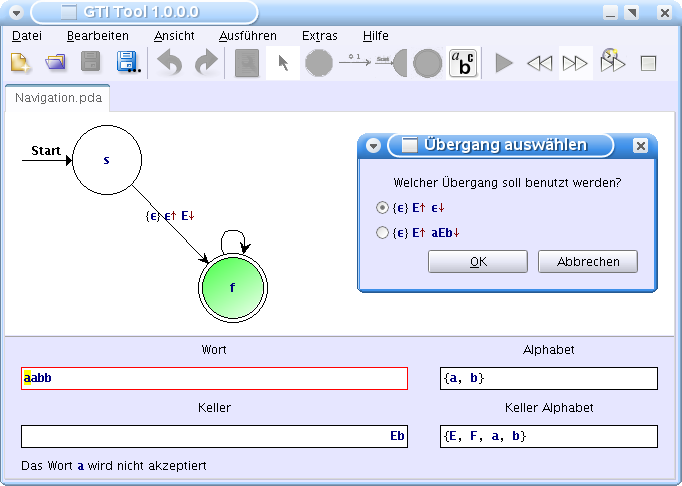
\includegraphics[width=12cm]{../images/grammar_pda.png}
\caption{Operationen mit dem Automaten Keller}
\end{center}
\end{figure}

Bei dem verwendeten Beispiel kommen zwei Übergänge in Frage. Es könnte der
Übergang gewählt werden, der \Symbol{E} vom Keller liest und nichts auf diesen
schreibt, oder aber der Übergang der \Symbol{E} vom Keller liest und
\Symbol{a}\Symbol{E}\Symbol{b} auf ihn schreibt. Da \Symbol{a} auf dem
Eingabeband steht, sollte der zweite Übergang ausgewählt werden. Dem Benutzer
steht es allerdings frei auch den anderen Übergang auszuwählen. In diesem Fall
würde das Wort \Symbol{a}\Symbol{a}\Symbol{b}\Symbol{b} aber nicht akzeptiert
werden. Der Benutzer hat bei einer falschen Wahl allerdings die Möglichkeit
einen oder mehrere Schritte zurückzugehen, um dann die richtige Wahl zu treffen.
